\documentclass[nooutcomes]{ximera}
\author{Jim Talamo and Bart Snapp}
\newcommand{\RR}{\mathbb R}
\renewcommand{\d}{\,d}
\newcommand{\dd}[2][]{\frac{d #1}{d #2}}
\renewcommand{\l}{\ell}
\newcommand{\ddx}{\frac{d}{dx}}
\newcommand{\dfn}{\textbf}
\newcommand{\eval}[1]{\bigg[ #1 \bigg]}



\outcome{Review the basic rules of differentiation and integration.}
\outcome{Review the relationship between differentiation and antidifferentiation.}
\outcome{Use algebra to manipulate the integrand.}
\outcome{Determine when a function is a composition of two or more functions.}
\outcome{Calculate indefinite and definite integrals requiring substitutions.}
\outcome{Recognize common patterns in substitutions.}
\outcome{Evaluate indefinite and definite integrals through a change of variables.}

%I want a separate section that reviews the FTC

\title[Dig-In:]{A review of integration}

\begin{document}
\begin{abstract}
  We review differentiation and integration.
\end{abstract}
\maketitle


\section{Review of derivative rules}

One of the fundamental objects of differential calculus is the \emph{derivative}.  As a reminder, here are some important results:

\index{derivative rules} 
  Let $n\ne 0$, $k$ be a constant and $a>0$.


\paragraph{Powers of $x$:}
\begin{itemize}
\item $\ddx k =0$
\item $\ddx x^n  = n x^{n-1}$
\end{itemize}

\paragraph{Exponentials:}
\begin{itemize}
\item $\ddx e^x = e^x$
\item $\ddx a^x = a^x\ln(a)$
\end{itemize}

\paragraph{Logartihms:}
\begin{itemize}
\item $\ddx \ln(x) = \frac{1}{x}$
\item $\ddx \log_a (x) = \frac{1}{\ln a} \frac{1}{x}$
\end{itemize}

\paragraph{Trigonometric Functions:}
\begin{itemize}
\item $\ddx \sin(x) = \cos(x)$
\item $\ddx \cos(x) = -\sin(x)$  
\item $\ddx \tan(x) = \sec^2(x)$  
\item $\ddx \sec(x) = \sec(x)\tan(x)$ 
\item $\ddx \csc(x) = -\csc(x)\cot(x)$
\item $\ddx \cot(x) = -\csc^2(x)$
\end{itemize}

\paragraph{Inverse Trigonometric Functions:}
\begin{itemize}
\item $\ddx \arcsin(x) = \frac{1}{\sqrt{1-x^2}}$
\item $\ddx \arccos(x) = \frac{-1}{\sqrt{1-x^2}}$
\item $\ddx \arctan(x) =\frac{1}{1+x^2}$
\item $\ddx \arcsec(x) = \frac{1}{|x|\sqrt{x^2-1}}$ for $|x|>1$
\item $\ddx \arccsc(x) = \frac{-1}{|x|\sqrt{x^2-1}}$ for $|x|>1$
\item $\ddx \arccot(x) = \frac{-1}{1+x^2}$
\end{itemize}



\begin{question} 
  Using the above rules only, what is the derivative of $\frac{1}{\sqrt[4]{x^3}}$ with respect to $x$?
  \begin{prompt} 
    \[
    \ddx \frac{1}{\sqrt[4]{x^3}} = \answer[given]{- \frac{3}{4} x^{-7/4}}
    \]
  \end{prompt}
\end{question}


Once the derivatives of basic functions have been established, we can use them to build the derivatives of more complicated functions:


\begin{theorem}[Derivatives of combinations of basic functions]
  Let $f(x)$ and $g(x)$ be differentiable functions.
\begin{itemize}
\item Addition: $\ddx \left( f(x) + g(x) \right) = f'(x) + g'(x)$
\item Scalar Multiplication: $\ddx \left( af(x) \right) = a f'(x)$
\item Product Rule: $\ddx \left( f(x) \cdot g(x) \right) = f(x)g'(x) + f'(x)g(x)$
\item Quotient Rule: $\ddx \frac{f(x)}{g(x)} = \frac{f'(x)g(x) - f(x)g'(x)}{(g(x))^2}$
\item Chain Rule: $\ddx f(g(x)) = f'(g(x)) \cdot g'(x)$
\end{itemize}
%\end{multicols}
\end{theorem}

%%%%%%%%%%%
\begin{question} 
  What is the derivative of $4x^2 +\frac{2}{3\sqrt{x}} $ with respect to $x$?
  \begin{prompt} 
    \[
    \ddx \left(4x^2 +\frac{2}{3\sqrt{x}} \right) = \answer[given]{8x -\frac{1}{3} x^{-3/2}}
    \]
  \end{prompt}
\end{question}

 %%%%%%%%%%%
 
%%%%%%%%%%%
\begin{question} 
  What is the derivative of $x^2 \sin(x) $ with respect to $x$?
  \begin{prompt} 
    \[
    \ddx x^2 \sin(x) = \answer[given]{2x \sin(x) +x^2 \cos(x)}
    \]
  \end{prompt}
\end{question}

 %%%%%%%%%%%
\begin{question} 
  What is the derivative of $\frac{e^x}{x^2+1}$ with respect to $x$?
  \begin{prompt} 
    \[
    \ddx \frac{e^x}{x^2+1} = \answer[given]{\frac{(- x^2 + 2x -1)e^x}{(x^2+1)^2}}
    \]
  \end{prompt}
 %%%%%%%%%%% 
\end{question}\begin{question} 
  What is the derivative of $\arcsin\left(\frac{x}{a}\right)$ with respect to $x$?
  \begin{prompt} 
    \[
    \ddx \arcsin\left(\frac{x}{a}\right) = \answer[given]{\frac{1}{a \sqrt{1-(x/a)^2}}}
    \]
  \end{prompt}
\end{question}





\section{Antiderivatives}


As a summary, one of the important questions of differential calculus is ``Given a function, what is its derivative?"  There is an important related question in integral calculus that requires ``undoing" the process of differentiation; that is, ``Given a function, what functions do we have to differentiate to obtain it?"   This is made precise by the following definition:

\begin{definition}\index{Antiderivative}  
Given a function $f(x)$, we say that $F(x)$ is an \dfn{antiderivative} of $f(x)$ if $F'(x) = f(x)$.
\end{definition}

 There is an important, but subtle way this definition is phrased; note that we used the phrase ``an antiderivative" and not ``the antiderivative".  To expound:
 
 \begin{question}
  Which of the following are antiderivatives of $2x$?
  \begin{selectAll}
    \choice[correct]{$x^2+5$}
    \choice[correct]{$x^2-3$}
    \choice{$2x^2+3$}
    \choice{$2-x^2$}
  \end{selectAll}
\end{question}

Notice that there are several choices for antiderivatives of $x^2$!  So, how could these antiderivatives differ?  The answer is a consequence of the Mean Value Theorem:
%%%Include exercise exploring MVT%%%%%%%
%%% Geometric reasoning %%%%%%

\begin{theorem}[Antiderivatives differ by a constant]
Let $f(x)$ be a function for which $F(x)$ and $G(x)$ are antiderivatives.  Then, there is a constant $C$ such that $F(x) = G(x) +C$. 
\end{theorem}

This theorem guarantees that the antiderivatives of a function $f(x)$ are the same up to an additive constant, which allows us to introduce the following notation:

%%%%%EXERCISE: integrate 1/(3x) two ways%%%%%%%%%%

\begin{definition}
Let $f(x)$ be a function.  The collection of \emph{all} antiderivatives of $f(x)$ is denoted by the symbol $\int f(x) \d x$. 
\end{definition}

%%%To summarize this, we review how to find $\int x^n \d x$ for $n \ne -1$:
%%
%%%To differentiate $x^n$:
%%%\begin{itemize}
%%\item Multiply by the current exponent $n$.
%%\item Subtract 1 from the exponent.
%%\end{itemize}
%%This process can be imagined with the flowchart: $$ x^n \longrightarrow nx^n \longrightarrow nx^{n-1} $$ %DOES XIMERA SUPPRT mathtools to put textover arrows %
%%
%%To find the collection of antiderivatives $\int x^n \d x$, first find \emph{an} antiderivative by reversing this process:
%%\begin{itemize}
%%\item Add 1 to the exponent.
%%\item Multiply by the reciprocal of the current exponent.
%%\end{itemize}
%%Now, to exhibit all of the antiderivatives, add an arbitrary constant.  This process can be imagined with the flowchart: $$ x^n \longrightarrow x^{n+1} \longrightarrow \frac{1}{n+1}x^{n+1}  \longrightarrow \frac{1}{n+1}x^{n+1} +C.$$
%%
Now it's your turn!

%%%%%%%%%%%%%%%%%%%%%

\begin{theorem}[Basic Indefinite Integrals]\index{antiderivatives}\index{indefinite integral}\hfil
\begin{itemize}
\item $\int k \d x= \answer[given]{k x}+C$
\item $\int \frac{1}{x} \d x= \answer[given]{\ln|x|}+C$
\item $\int x^n \d x= \answer[given]{\frac{x^{n+1}}{n+1}}+C\qquad(n\ne-1)$
\item $\int e^x \d x= \answer[given]{e^x} + C$
\item $\int a^x \d x= \answer[given]{\frac{a^x}{\ln(a)}}+C$
\item $\int \cos(x) \d x = \answer[given]{\sin(x)} + C$
\item $\int \sin(x) \d x = \answer[given]{-\cos(x)} + C$  
\item $\int \sec^2(x) \d x = \answer[given]{\tan(x)} + C$
\item $\int \csc^2(x) \d x = \answer[given]{-\cot(x)} + C$
\item $\int \sec(x)\tan(x) \d x = \answer[given]{\sec(x)} + C$
\item $\int \csc(x)\cot(x) \d x = \answer[given]{-\csc(x)} + C$
\item $\int \frac{1}{x^2+a^2}\d x = \answer[given]{\frac{1}{a}\arctan\left(\frac{x}{a}\right)} + C$
\item $\int \frac{1}{\sqrt{a^2-x^2}}\d x= \answer[given]{\arcsin\left(\frac{x}{a}\right)}+C$
\end{itemize}
\end{theorem}

%%%%%%%%%%%%

Unfortunately, many of the helpful rules that allow us to find derivatives of more complicated functions are not easily reversible.  We do have the following:

\begin{theorem}[Antiderivative Rules] 
Suppose that $f(x)$ and $g(x)$ are functions and $a$ is a constant:
\begin{itemize}
\item (Addition) $\int \left(f(x) + g(x) \right) \d x = \int f(x) \d x+\int g(x)  \d x$
\item (Scalar Multiplication) $\int \left(a f(x)\right) \d x = a \int f(x) \d x$
\end{itemize}
\end{theorem}

%%%%%%%%%%%
\begin{question} 
  Find $\int \left(4x^2 + \dfrac{1}{1+x^2} \right)\d x$.
  \begin{prompt} 
    \[
    \int \left(4x^2 + \dfrac{1}{1+x^2} \right) \d x  = \answer[given]{\frac{4}{3} x^3 + \arctan(x)} +C 
    \]
  \end{prompt}
\end{question}

 %%%%%%%%%%%


Unfortunately, there is no rule that allows us to compute antiderivatives of products, quotients, or compositions of arbitrary functions based off of the antidifferentiation formulas for their constituent functions as there is with differentiation!  


\begin{example}
  A student claims that $\int 2x \cos^x \d x = x^2 \sin(x) +C$.  Determine whether the student is correct or incorrect.
  
  \begin{explanation}
    If the student were correct, then the derivative of $x^2 \sin(x) +C$ with respect to $x$ would have to be $2x \cos^x$.  However:
    
      \[\ddx x^2 \sin(x) = \answer[given]{2x \sin(x) +x^2 \cos(x)} \]
      
 Hence, the student is incorrect!
  \end{explanation}
\end{example}

\begin{remark}
Finding antiderivatives is an integral part of integral calculus!  If you are unsure whether you have found the correct antiderivatives of a function, you should check your work simply by taking the derivative of your proposed antiderivative!  
\end{remark}

\begin{question}
  Consider $f(x) = \cos(\sqrt{x})$. Which of the following is $\int f(x) \d x$?  
  \begin{selectAll}
    \choice{$\sin(\sqrt{x}) +C$}
    \choice{$\dfrac{1}{\sqrt{x}}\sin(\sqrt{x}) +C$}
    \choice{$-\dfrac{1}{2 \sqrt{x}} \sin (\sqrt{x})$}
    \choice[correct]{$2 \cos(\sqrt{x}) + 2 \sqrt{x} \sin(\sqrt{x}) +C$}
    \choice{None of these}
  \end{selectAll}
\end{question}

The following is a question that employs the same logic, but is phrased a bit differently:

\begin{example}
  Find a function $f(x)$ such that $\int f(x) \d x = x^2 +C$.
  
  \begin{explanation}
    We are looking for a function $f(x)$ whose \emph{antiderivatives} are $x^2+C$.  To do this, we simply have to take the derivative of the righthand side; since $\int f(x) \d x =x^2+C$, then $f(x) = \ddx(\answer[given]{x^2+C}) =\answer[given]{2x}$.
    
    \end{explanation}
\end{example}

Now, you try!

\begin{question} 
  Find a function $f(x)$ such that $\int f(x) \d x = xe^x +C$.

  \begin{prompt} 
    \[
    f(x) = \answer[given]{e^x + xe^x}
    \]
  \end{prompt}
\end{question}
%%%%%%%%%END%%%%%%%%

Whenever you compute an indefinite integral, you can always check your
work by taking the derivative. In particular, this means that if you
are given choices for the antiderivative, you can check . Note, there are always many choices for
antiderivative, as they may differ by a constant.

%\begin{question}
  %Which of the following are an antiderivative of $\frac{1}{x\ln(x^2)}$?
  %\begin{selectAll}
    %\choice[correct]{$\frac{1}{2}\ln(\ln(x^2))$}
    %\choice[correct]{$\frac{\ln(2) + \ln(\ln(x))}{2}$}
    %\choice[correct]{$\frac{\ln(\ln(x))}{2}$}
    %\choice[correct]{$\frac{\ln(7\cdot \ln(x))}{2}$}
    %\choice[correct]{$\frac{\ln(\ln(x^3))}{2}$}
  %\end{selectAll}
%\end{question}

%%%%%%%%%%%%%%%Exercises%%%%%%%%%%%%%%

\section{Definite Integrals}
For continuous functions, the Fundamental Theorem of Calculus provides the link between the process of antidifferentiation and finding certain areas.  This will be reviewed in a subsequent section, but we review how to compute definite integrals of continuous functions here:

\begin{theorem}[Fundamental Theorem of Calculus]\index{Fundamental Theorem of Calculus}
  Let $f$ be continuous on $[a,b]$. If $F$ is \textbf{any}
  antiderivative of $f$, then
  \[
  \int_a^b f(x)\d x = F(b)-F(a).
  \]
\end{theorem}

\begin{example}
Calculate $\int_0^{\ln(3)} 2e^x \d x.$  We find the antiderivative first, then evaluate the expression given by the Fundamental Theorem of Calculus:

\begin{align*}
\int_0^{\ln(3)} 2e^x \d x &= \eval{2e^x}_0^{\ln(3)} \\
&= 2e^{\ln(3)}-2e^0 \\
&= 2(3) -2 \\
&= 4
\end{align*}
\end{example}

%%%%%%%%%%%%%%%%%%%%%%%%%%%%%%



\section{Common techniques for finding antiderivatives}
In some sense, calculating derivatives is ``easy".  Most of the functions that you've studied so far are sums, scalar multiples, products, quotients, or compositions of the functions listed at the beginning of this section.  A ``brute force" application of the sum, scalar multiple, product, quotient, and chain rules will eventually lead to a correct derivative.  Integration is more of an art form.  We often have to apply various techniques in order to write down a nice formula for the antiderivatives. We explore some of the common ones here:

\section{Preliminary algebra}

A good first step in attempting to compute antiderivatives involves simplifying the integrand first.  Make sure you are careful when doing algebra!


\begin{example}
  Compute:
  \[
  \int (7-x^2)^2 \d x
  \]
  \begin{explanation}
    Let's start by expanding the integrand:
    \[
    \int (7-x^2)^2 \d x  = \int \answer[given]{49 - 14x^2 + x^4} \d x
    \]
    Ah, this is now easy, write with me:
    \[
    \int 49 - 14x^2 + x^4 \d x = \answer[given]{49x - \frac{14 x^3}{3} + \frac{x^5}{5}} + C
    \]
  \end{explanation}
\end{example}

\begin{example}
Consider the indefinite integral $\int \sqrt{x}(x+1)^2 \d x$.  

While it may be tempting, note that $\sqrt{x}(x+1)^2 \neq (\sqrt{x}(x+1))^2$ by order of operations (exponentiation comes first). Instead, we can expand $(x+1)^2 = \answer[given]{x^2+2x+1}$ and rewrite the integrand:

\begin{align*}
\int \sqrt{x}(x+1)^2 \d x &= \int x^{1/2} (x^2+2x+1) \d x \\
&=  \int x^{5/2}+2x^{3/2}+x^{1/2} \d x \\
&= \frac{2}{7} x^{7/2}+\frac{4}{5}x^{5/2}+\frac{2}{3}x^{3/2}+C
\end{align*}

\end{example}
 
\begin{example}
Consider the indefinite integral $\int \frac{2x^2-3}{2x^2} \d x$.  

While it may be tempting, note that $\frac{2x^2-3}{2x^2} \neq \frac{\cancel{2x^2}-3}{\cancel{2x^2}}$!  We can never simplify by cancelling terms over addition or subtraction!  Instead, we can split the fraction up then simplify: 
\begin{align*}
\int \frac{2x^2-3}{2x^2} \d x &=\int \frac{2x^2}{2x^2}-\frac{3}{2x^2} \d x \\
&=  \int 1+\frac{3}{2}x^{-2} \d x \\
&= x- \answer[given]{\frac{3}{2}x^{-1}}+C
\end{align*}

\end{example}

  
\section{Substitution}

While some integrands involve complicated expressions that cannot be simplified algebraically, a change of variable can often help. Often, when an integrand involves a composition of a trigonometric, exponential, or power and another function, letting a new variable represent the inner function helps!

\begin{example}
Consider $\int 2x e^{x^2+1} \d x$.  

Note that no algebra will help us simplify the expression.  The only antidifferentiation formula we have regarding the exponential is $\int e^x \d x = e^x +C$.  Let's start by letting the exponent in the original integral be a new variable $u$:

Let $u= x^2+1$.  We now need to write everything in the integral in terms of this new variable.  Recalling that if $u = f(x)$, the differentials are related by $\d u = f'(x) \d x$, we can write $\d u = \answer[given]{2x} \d x$, or solving for $\d x$, we find $\d x = \answer[given]{\frac{1}{2x}} \d u$.

Thus, $\int 2x e^{x^2+1} \d x = \int 2x e^{u} \frac{1}{2x} \d u = \int e^u \d u$.

The antiderivative in $u$ is now easy to compute!  Indeed:

\[ \int e^u \d u = \answer[given]{e^u}+C \]

We now substitute for $u$ to finish:

\[\int 2xe^{x^2+1} \d x = e^u+C = e^{\answer[given]{x^2+1}}+C \]

\end{example}


Sometimes, the substitutions involve some preliminary algebra:

\begin{example} 

  Letting $a>0$, compute:
  \[
  \int \frac{1}{\sqrt{a-x^2}} \d x
  \]
  \begin{explanation}
    Looking over our basic integral formulas, we see that this is similar to
    \[
    \int \frac{1}{\sqrt{1-x^2}}\d x= \answer[given]{\arcsin(x)}+C.
    \]
    So our goal will be to somehow ``transform'' the integral we are
    trying to compute to one that is similar to the one we know how to
    compute. First note:
    \[
    \int \frac{1}{\sqrt{a-x^2}} \d x  =
    \int \frac{1}{\sqrt{\answer[given]{a}\left(1-\frac{x^2}{a}\right)}} \d x
    \]
    and since $a>0$, we may write:
    \[
    \int \frac{1}{\sqrt{a\left(1-\frac{x^2}{a}\right)}} \d x=
    \int \frac{1}{\answer[given]{\sqrt{a}}\cdot \sqrt{1-\left(\frac{x}{\sqrt{a}}\right)^2}} \d x
    \]
    Recalling that we may always pull constants out of integrals, write:
    \[
    \int \frac{1}{\sqrt{a}\cdot \sqrt{1-\left(\frac{x}{\sqrt{a}}\right)^2}} \d x = 
    \answer[given]{\frac{1}{\sqrt{a}}}\int \frac{1}{\sqrt{1-\left(\frac{x}{\sqrt{a}}\right)^2}} \d x 
    \]
    Ah! Now our integral looks more like one we can do. We will now
    proceed using substitution. Set $u = \frac{x}{\sqrt{a}}$, and write with me
    \begin{align*}
      \d u &= \frac{\d x}{\sqrt{a}},\\
      \d x &= \sqrt{a}\d u,
    \end{align*}
    and now
    \begin{align*}
    \frac{1}{\sqrt{a}}\int \frac{1}{\sqrt{1-\left(\frac{x}{\sqrt{a}}\right)^2}} \d x &=
    \frac{1}{\sqrt{a}}\int \frac{1}{\sqrt{1-u^2}} \sqrt{a} \d u\\
    &=\int \frac{1}{\sqrt{1-u^2}}\d u\\
    &=\arcsin(u) + C\\
    &=\arcsin\left(\frac{x}{\sqrt{a}}\right) + C.
    \end{align*}
  \end{explanation}
\end{example}

%%%EXERCISE: WHY NOT A COMPUTER? \int x(x+1)^50%%%%



\begin{question}
  Letting $a$ be nonzero, what is the antiderivative of $\frac{1}{a +
    x^2}$?
  \begin{prompt}
    \[
    \int \frac{1}{a + x^2} \d x = \answer[given]{\frac{1}{\sqrt{a}} \arctan\left(\frac{x}{\sqrt{a}}\right)}+C
    \]
  \end{prompt}
  \begin{hint}
    Try to use the same procedure used in the example above.
  \end{hint}
\end{question}


Let's see another example involving a trickier substitution and a definite integral.  First, recall the substitution theorem for definite integrals:

\begin{theorem}[Integral Substitution Formula] 
If $g$ is differentiable on the interval $[a,b]$ and $f$ is
differentiable on the interval $[g(a),g(b)]$, then
\[
\int_a^b f'(g(x)) g'(x) \d x =\int_{g(a)}^{g(b)} f'(g) \d g.
\]
\end{theorem}

This reminds us that to work with definite integrals, we need to write the integrand, the differential, and the limits of integration in terms of the new variable!  

\begin{example}
Compute:
\[
\int_0^{16} \sqrt{4 - \sqrt{x}} \d x
\]
\begin{explanation}
To make the integral appear a little nicer, let us try the substitution
\[
u = \sqrt{x}.
\]
Then:
\begin{align*}
\d u &= \answer[given]{\frac{1}{2 \sqrt{x}}} \d x,\\
\d x &= 2 \sqrt{x} \d u = 2u \d u,
\end{align*}
where we used the fact that $u=\sqrt{x}$ in the last equality.  So:
\begin{align*}
\int_{x=0}^{x=16} \sqrt{4 - \sqrt{x}} \d x &=  \int_{u=\answer[given]{0}}^{u=\answer[given]{4}} \answer[given]{2u \sqrt{4-u}} \d u.
\end{align*}
From here we now make the second (and more obvious) substitution
\[
v = 4-u.
\]
Then $u = 4-v$, and: 
\begin{align*}
\d v &= - \d u,\\
\d u &= - \d v.
\end{align*}
So:
\begin{align*}
\int_{x=0}^{x=16} \sqrt{4 - \sqrt{x}} \d x &= \int_{u=0}^{u=4} 2u \sqrt{4-u} \d u  \\
&= \int_{v=\answer[given]{4}}^{v=\answer[given]{0}} 2 (4-v) \sqrt{v} (-1) \d v  \\
&= \int_{v=\answer[given]{4}}^{v=\answer[given]{0}} 2v^{\frac{3}{2}} - 8v^{\frac{1}{2}}  \d v  \\
&= \eval{ \answer[given]{  \frac{4}{5} v^{\frac{5}{2}} -  \frac{16}{3} v^{\frac{3}{2}} }}_{4}^{0}  \\
&=  \left( 0 - 0 \right) - \left(\frac{4}{5} (4)^{\frac{5}{2}} - \frac{16}{3} (4)^{\frac{3}{2}}  \right)   \\
&= \frac{128}{3} - \frac{128}{5}   \\
&= \frac{256}{15}.
\end{align*}
\end{explanation}
\end{example}


%\section{Algebra to the rescue} <-----MOVE TO ANOTHER SECTION

%With substitution, and a little algebraic manipulation, one can
%compute more integrals. In what follows, we will work many examples.
%In each case below we will present a ``novel'' integral, and then use
%algebra and substitution to change the form of the integral to one
%we know.



%Functions consisting of products of the sine and cosine can be
%integrated by using substitution and trigonometric identities. These
%can sometimes be tedious, but the technique is straightforward. The
%basic idea in each case is to somehow take advantage of a
%trigonometric identity, usually the Pythagorean identity, or a
%power-reduction formula:
%\begin{description}\index{Pythagorean identity}\index{power-reduction!formula}
%\item[Pythagorean Identity] $\cos^2(x) + \sin^2(x) = 1$
%\item[Cosine Power-Reduction] $\cos^2(x)= \frac{1+\cos(2x)}{2}$\index{cosine power-reduction}
%\item[Sine Power-Reduction] $\sin^2(x) = \frac{1-\cos(2x)}{2}$\index{sine power-reduction}
%\end{description}

%We'll work some examples to demonstrate how to use these formulas.

%\begin{example}
%  Compute:
%  \[
%  \int (\cos(x)+\sin(x))^2\d x
%  \]
 % \begin{explanation}
 %   Let's start by expanding the integrand:
%    \begin{align*}
%      \int &(\cos(x)+\sin(x))^2 \d x\\
%      &= \int \answer[given]{\cos^2(x) + 2\cos(x)\sin(x) + \sin^2(x)} \d x
%    \end{align*}
 %   Now if we rearrange we can use the Pythagorean identity, write with me:
 %   \begin{align*}
 %     \int &\cos^2(x) + 2\cos(x)\sin(x) + \sin^2(x) \d x \\
%      &= \int \cos^2(x) + \sin^2(x) + 2\cos(x)\sin(x) \d x\\
 %     &= \int \answer[given]{1 + 2\cos(x)\sin(x)} \d x
  %  \end{align*}
%    Now we may set $g = \sin(x)$ and so
 %   \begin{align*}
 %     \d g &= \answer[given]{\cos(x)} \d x,\\
 %     \d x & = \frac{\d g}{\cos(x)},
%    \end{align*}
 %   and we find
 %   \begin{align*}
 %     \int 1 + 2\cos(x)\sin(x) \d x &= \int 1 \d x + \int 2g \d g\\
%      &= x + g^2 + C\\
%      &= x + \answer[given]{\sin^2(x)}+C.
 %   \end{align*}
%  \end{explanation}
%\end{example}

\begin{comment}
Let's see one more example with trigonometric functions:

\begin{example}
  Compute:
  \[
  \int \frac{\sin(x) + \cos^2(x)}{\csc(x)} \d x
  \]
  \begin{explanation}
    To start, let's express everything in terms of sine and cosine:
    \begin{align*}
      \int \frac{\sin(x) + \cos^2(x)}{\csc(x)} \d x &= \int \frac{\sin(x) + \cos^2(x)}{\frac{1}{\sin(x)}} \d x\\
      &= \int \sin^2(x) + \sin(x)\cos^2(x) \d x
    \end{align*}
    if we use our power-reduction formula above, we find
    \[
    \int \answer[given]{\frac{1-\cos(2x)}{2}}+ \sin(x)\cos^2(x) \d x
    \]
    Splitting this integral up we now have
    \begin{align*}
      \int &\answer[given]{\frac{1}{2}} \d x - \int \frac{\cos(2x)}{2}\d x + \int \sin(x)\cos^2(x) \d x  \\
      &= \answer[given]{\frac{x}{2} - \frac{\sin(2x)}{4} - \frac{\cos^3(x)}{3}}+C.
    \end{align*}
  \end{explanation}
\end{example}
\end{comment}

\section{Splitting Up Fractions}

In a similar vein, if you have a rational function, it can help to separate the
integrand into several fractions.

\begin{example}
  Compute:
  \[
  \int \frac{6x-8}{1+x^2}\d x
  \]
 
  \begin{explanation}
    Note that the substitution $u= 1+x^2$ is tempting, but it only will help us with part of the integrand!  Write with me:
    \[ \int \frac{6x-8}{1+x^2}\d x = \int \frac{6x}{1+x^2}-\frac{8}{1+x^2} \d x \]
      
Using a substitution, $ \int \frac{6x}{1+x^2}\d x = \answer[given]{3 \ln(1+x^2)}$+C, and using the inverse tangent antidifferentiation formula, $ \int \frac{8}{1+x^2}\d x = \answer[given]{8 \arctan(x)}$+C.

Hence, $\int \frac{6x-8}{1+x^2}\d x =  \answer[given]{3 \ln(1+x^2)- 8 \arctan(x)}+C$
  \end{explanation}
\end{example}

\begin{example}
  Compute:
  \[
  \int \frac{\cos^2(x)+1}{3 \cos^2(x)}\d x
  \]
 
  \begin{explanation}
    Write with me:
    \begin{align*}
    \int \frac{\cos^2(x)+1}{3 \cos^2(x)}\d x &=  \int \frac{\cos^2(x)}{3 \cos^2(x)} +  \frac{1}{3 \cos^2(x)}\d x \\
    &= \int \frac{1}{3} + \frac{1}{3} \sec^2(x) \d x \\
    & = \answer[given]{\frac{1}{3}x+\frac{1}{3}\tan(x)}+C 
    \end{align*}
      
  \end{explanation}
\end{example}


\section{Other Techniques}
Your old friend (or enemy!) long-division\index{long-division} can help too.

\begin{example}
  Compute:
  \[
  \int \frac{3x^2-17x +1}{x-5} \d x
  \]
  \begin{explanation}
    Now we will use long-division. Write:
    %%\[
    %% x-5\,\begin{array}[b]{@{}r@{}r} 
    %% \answer[given]{3x-2} &\\ 
    %% \cline{1-1}
    %% \Bigg)\begin{array}[t]{@{}l@{}} 3x^2-17x+1\\ 
    %%   \answer[given]{3x^2-15x} \\ 
    %%   \divrule{0}{8}  ~~~~~\answer[given]{-2x+1} \\
    %%   ~~~~~\answer[given]{-2x+10}\\
    %%   \divrule{5}{8}
    %%   ~~~~~~~~~~\answer[given]{-9}
    %% \end{array}
    %% \end{array}
    %% \]
    \begin{center}%%BADBAD
      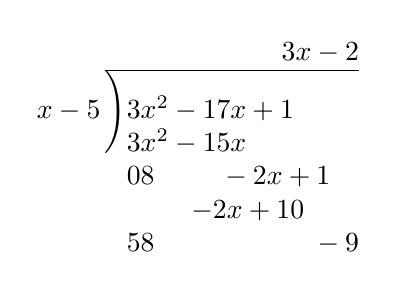
\begin{tikzpicture}[]
        \node at (0,0) {
    $x-5\,\begin{array}[b]{@{}r@{}r} 
    3x-2 &\\ 
    \cline{1-1}
    \Bigg)\begin{array}[t]{@{}l@{}} 3x^2-17x+1\\ 
      3x^2-15x \\ 
      \divrule{0}{8}  ~~~~~~~-2x+1 \\
      ~~~~~~~-2x+10\\
      \divrule{5}{8}
      ~~~~~~~~~~~~~~~~~-9
    \end{array}
    \end{array}
          $
        };
      \end{tikzpicture}
    \end{center}
    From this we see that
    \begin{align*}
      \int \frac{3x^2-17x +1}{x-5} \d x &= \int 3x-2 - \answer[given]{\frac{9}{x-5}}\d x\\
      &= \frac{3x^2}{2} - 2x -9 \ln|x-5| +C
    \end{align*}
    %Why is the rendering wrong?
  \end{explanation}
\end{example}

Finally, sometimes it helps to complete the square.\index{complete the square}

\begin{example}
  Compute:
  \[
  \int \frac{1}{x^2-17x +1}\d x
  \]
  \begin{explanation}
    To start, let's complete the square in the denominator. Write with me:
    \begin{align*}
      \int &\frac{1}{x^2-17x +1} \d x \\
      &=  \int \frac{1}{x^2-17x +\left(\frac{17}{2}\right)^2 + 1 - \left(\frac{17}{2}\right)^2} \d x\\
      &=  \int \frac{1}{\left(\answer[given]{x-\frac{17}{2}}\right)^2 + 1 - \left(\frac{17}{2}\right)^2} \d x
    \end{align*}
    At this point set $u= x-\frac{17}{2}$, so $\d u = \d x$ and we have
    \begin{align*}
    \int &\frac{1}{u^2 + 1 - \left(\frac{17}{2}\right)^2} \d u \\
    &= \frac{1}{\sqrt{1 - \left(\frac{17}{2}\right)^2}} \arctan\left(\frac{u}{\sqrt{1 - \left(\frac{17}{2}\right)^2}}\right)\\
    &= \frac{1}{\sqrt{1 - \left(\frac{17}{2}\right)^2}} \arctan\left(\frac{\answer[given]{x-\frac{17}{2}}}{\sqrt{1 - \left(\frac{17}{2}\right)^2}}\right).
    \end{align*}
  \end{explanation}
\end{example}

As you can see, integration is often far more challenging than differentiation.  Concerted time and practice are needed to become familiar with the necessary technique or techniques required to evaluate antiderivatives.  As a final strategy, please, when you are learning, feel free to find
the answer using a computer. While this may seem like ``cheating'' but you
can gain insight from it as long as you make sure you understand how to obtain the answer! 
\begin{quote}
  \textbf{Always remember: Don't give up.}
\end{quote}
\end{document}
